\input{preamble.txt}


\begin{document}

\section{Object Oriented Programming (2)}

\begin{itemize}
	\item Abstract Classes
	\begin{itemize}
		\item Cannot be instantiated using the \textbf{new} operator
		\item Usually contain abstract methods that are implemented in concrete subclasses
		\begin{itemize}
			\item e.g. computeArea() in GeometricObject
		\end{itemize}
		\item Abstract classes and abstract methods are denoted using the
		\textbf{abstract} modifier in the header
		\item A class that contains abstract methods must be defined as abstract
		\item If a subclass of an abstract superclass does not implement all the abstract methods, the subclass must be defined as abstract
	\end{itemize}

	\item Interfaces
	\begin{itemize}
		\item An interface can be used to define common behaviour for classes (including unrelated classes)
		\item Contains only constants and abstract methods
		\item Interfaces are denoted using the \textbf{interface} modifier in the header
		\item Example\\
		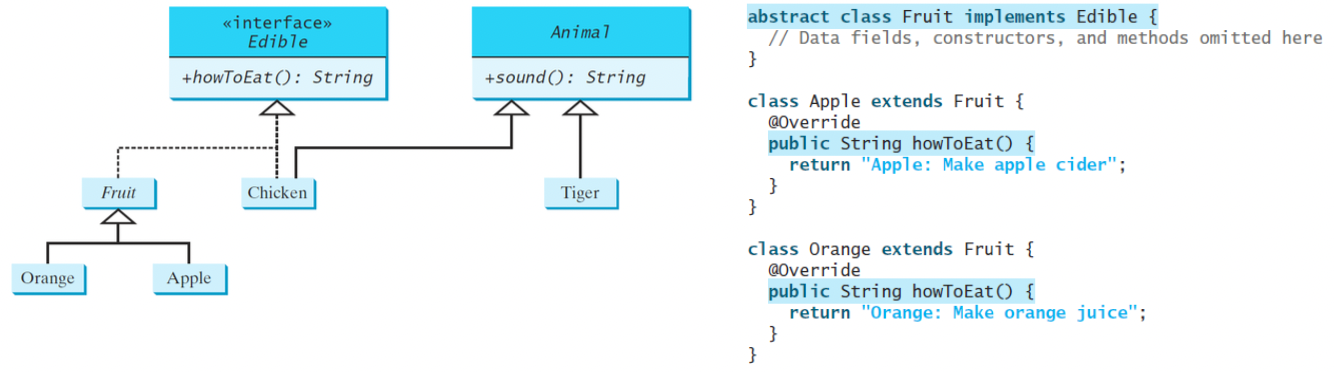
\includegraphics[scale=0.7]{Interface.png}
	\end{itemize}

	\item Generics
	\begin{itemize}
		\item Enable type parameterization
		\begin{itemize}
			\begin{minipage}[h]{\widthof{Generic interfaces} + 1cm}
				\item Generic interfaces
			\end{minipage}
			\begin{minipage}[h]{\widthof{Generic classes} + 1cm}
				\item Generic classes
			\end{minipage}
			\begin{minipage}[h]{\widthof{Generic methods} + 1cm}
				\item Generic methods
			\end{minipage}
		\end{itemize}
		\item Example: \textbf{ArrayList} class
		\begin{itemize}
			\item ArrayList$\langle$Integer$\rangle$ A = new ArrayList$\langle$Integer$\rangle$();
			\item ArrayList$\langle$String$\rangle$ B = new ArrayList$\langle$String$\rangle$();
		\end{itemize}
		\item Generic types must be reference types
		\item Enable error detection at compile time
		\item The \textbf{Comparable} interface
		\begin{itemize}
			\item Defines the \textbf{compareTo} method for comparing objects
			\item Defined as follows:\\[5pt]
			\begin{minipage}{0.5\textwidth}
				\begin{Verbatim}
		public interface Comparable<T> {
			public int compareTo(T t);
		}
				\end{Verbatim}
			\end{minipage}
			\item The \textbf{compareTo} method determines the order of the calling object with \textbf{t} and returns a negative integer, zero, or a positive integer if the calling object is less than, equal to, or greater than \textbf{t}
			\item Many classes implement Comparable (e.g. \textbf{String}, \textbf{Integer})
		\end{itemize}
		%			\newpage
		\item The \textbf{ArrayList} class
		\begin{itemize}
			\item Arrays can be used to store lists of objects. However, once an
			array is created, its size is fixed
			\item Java provides the generic class \textbf{ArrayList} whose size is variable
			\item Imported using: \textbf{import java.util.ArrayList;}
			\item Commonly used methods (\textbf{ArrayList<E>})
			\begin{itemize}
				\item \textbf{boolean add(E e)}
				\item \textbf{E get(int index)}
				\item \textbf{int size()}
				\item \textbf{boolean contains(Object o)}
				\item \textbf{int indexOf(Object o)}
			\end{itemize}
			\item An \textbf{ArrayList} could be traversed using a for-each loop
		\end{itemize}
%		\newpage
		\item The \textbf{HashSet} class
		\begin{itemize}
			\item Generic class that can be used to store elements without duplicates
			\begin{itemize}
				\item No two elements e1 and e2 can be in the set such that e1.equals(e2) is true
			\end{itemize}
			\item Imported using: \textbf{import java.util.HashSet;}
			\item Objects added to the hash set should override \textbf{equals} and \textbf{hashCode} properly
			\item Commonly used methods (\textbf{HashSet$\langle$E$\rangle$})
			\begin{itemize}
				\item \textbf{boolean add(E e)}
				\item \textbf{int size()}
				\item \textbf{boolean contains(Object o)}
			\end{itemize}
			\item A \textbf{HashSet} could be traversed using a for-each loop
		\end{itemize}

		\item The \textbf{LinkedHashSet} class
		\begin{itemize}
			\item Elements of a \textbf{HashSet} are not necessarily stored in the same
			order they were added
			\item \textbf{LinkedHashSet} is a subclass of \textbf{HashSet} with a linked-list implementation that supports an ordering of the elements in the set
			\item Imported using: \textbf{import java.util.LinkedHashSet;}
		\end{itemize}
	\end{itemize}

	\item Exceptions
	\begin{itemize}
		\item Example\\
		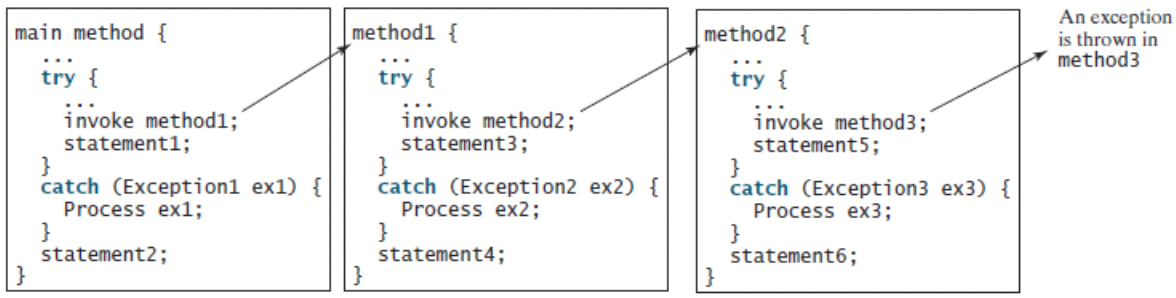
\includegraphics[scale=0.7]{Exceptions.png}
		\item Java has a \textbf{finally} clause that can be used to execute some code regardless of whether an exception occurs or is caught. For example:
		\begin{Verbatim}
			try {
				//statements;
			}
			catch Exception ex) {
				//handling ex; }
			finally {
				//final statements;
			}
		\end{Verbatim}
	\end{itemize}
\end{itemize}
\newpage

\subsection*{Object Oriented Programming - Design Guidelines}
\begin{itemize}
	\item Methods Common to All Objects
	\begin{itemize}
		\item Always override hashCode when you override equals
		\item Always override toString
		\item ConsiderimplementingComparable
	\end{itemize}

	\item Classes and Interfaces
		\vspace{9pt}
		\begin{itemize}
		\begin{minipage}[h]{\widthof{Favor composition over inheritance} + 1cm}
			\item Minimize accessibility
			\item Favor composition over inheritance
		\end{minipage}
		\begin{minipage}[h]{0.4\textwidth}
			\item Prefer interfaces to abstract classes
			\item Prefer lists to arrays
		\end{minipage}
		\end{itemize}


	\item Methods
	\begin{itemize}
		\item Check parameters for validity
		\item Return empty arrays or collections, not \textbf{null}
		\item Document your API properly
	\end{itemize}

	\item Exceptions
	\begin{itemize}
		\item Use exceptions only for exceptional conditions
		\item Use checked exceptions for recoverable conditions and runtime exceptions for programming errors
		\item Do not ignore exceptions
	\end{itemize}

	\item General Programming (Naming Conventions)
	\begin{itemize}
		\item Package names should be hierarchical with the components separated by periods. Components should consist of lowercase alphabetic characters and, rarely, digits. e.g. \textbf{javax.swing.plaf.metal}
		\item Class and interface names should consist of one or more words, with the first letter of each word capitalized
		\item Method and field names follow the same typographical conventions as class and interface names, except that the first letter of a method or field name should be lowercase, for example, \textbf{ensureCapacity}
		\item The names of constant fields should consist of one or more uppercase words separated by the underscore character, for example, \textbf{NEGATIVE\textunderscore INFINITY}
		\item Local variable names have similar typographical naming conventions to member names, except that abbreviations are permitted, as are individual characters and short sequences of characters whose meaning depends on the context in which the local variable occurs, for example, \textbf{i}, \textbf{xref}
	\end{itemize}
\end{itemize}
\end{document}